\chapter{Přístupnost na webu}

Tato kapitola se věnuje představení problematice přístupnosti na webu.

\section{Přístupný web}

Přístupnost na webu je definována jako schopnost webového obsahu být interpretován a používán nejširším možným spektrem uživatelů bez ohledu na jejich schopnosti, nebo fyzický stav~\cite{w3-accessibility}.

\subsection{Kategorizace postižení}

Moderní internet je plný různorodého multimediálního obsahu a každý má svá specifika, které ho můžou dělat nepřístupným, nebo i přístupným pro určitou skupinu uživatelů.
Mezi nejčastější a prozkoumané kategorie patří~\cite{w3-disabilities}:

\begin{itemize}
  \item \textbf{Vizuální} --- Barvoslepost, zhoršené vidění či úplná slepota.
        Je důležité udržovat pravidla správného kontrastu barev a správné velikosti písma, nebo minimálně umožnit uživateli tyto hodnoty změnit.
  \item \textbf{Sluchové} --- Částečně zhoršené slyšení, nebo úplná hluchota v jednom či obou uších.
        Média, která využívají zvuk pro přenos informací je potřeba doplnit o možnosti změny hlasitosti, nebo doplnění o textový přepis či titulky.
  \item \textbf{Motorické} --- Chybějící končetina, třes, zhoršená koordinace a paralýza.
        Pro uživatele s motorickými postiženími je důležité mít přístupné ovládání pomocí klávesnice.
        Uživatelé využívají alternativních zařízení pro manipulaci s obsahem webu jako jsou ergonomické příslušenství, ústní myš, trackbally a další.
        Přístupnost přes klávesnici velice často pomáhá zmíněným zařízením fungovat dle potřeby uživatele.
  \item \textbf{Kognitivní} --- Kognitivní potíže mohou zasáhnout některou část nervové soustavy člověka.
        Ať už je to vnímaní informací, paměť, učení čí porozumění.
        V kontextu webu je důležité informace prezentovat nejjednodušším, jasným způsobem a nechat uživatelům dostatek času na pochopení a reakci.
\end{itemize}

Mezi další kategorie postižení patří například poruchy řeči, ale v kontextu této práce se jimi nebudu zabývat, neboť nejsou relevantní pro tvorbu znovupoužitelných komponent.

\section{W3C a WAI}

% TODO: Potřebuje poupravit slova.

\gls{w3c}\footnote{\url{https://www.w3.org}} je mezinárodní konsorcium, které vyvíjí standardy pro web.
\gls{wai} je jedním z projektů \gls{w3c}, který se zaměřuje na přístupnost webu.
WAI definuje specifikace a doporučení pro mnohé aspekty přístupnosti na webu, od \textit{user agentů}, evaluačních nástrojů až po nástroje pro tvorbu digitálního obsahu.

\section{WAI-ARIA}

\gls{waiaria}\footnote{\url{https://www.w3.org/TR/wai-aria}} je technická specifikace, která rožšiřuje webové technologie (HTML, JavaScript, Ajax) o ontologii atributů představující role, vlastnosti a stavy elementů~\cite{wai-aria}.
Zmíněné atributy umožňují asistivním technologiím (například čtečky obrazovky) předat uživatelům význam a podrobnější informace o elementech, které se nachází na daném webu a tím jim pomoci s pochopením a manipulací obsahu stránky.

\subsection{ARIA role}

Role slouží k přidání sémantického významu HTML elementům tak, aby nevidomí či uživatelé s jinou formou postižení dokázali pochopit účel daného elementu.

Některé HTML elementy mohou mít svůj sémantický význam i bez použití rolí~\cite{wai-implicit-semantics}.
Například \textit{button} element se používá pro interaktivní tlačítka a je vhodnější jej použít namísto nesémantického divu s rolí button.

\clearpage

\begin{lstlisting}[caption={Aria role}, label={aria-roles}, language=html]
<ul role="menu">(*@\label{aria-roles-1}@*)
  <li role="menuitem">Open file</li>(*@\label{aria-roles-2}@*)
  <li role="menuitem">Save file</li>(*@\label{aria-roles-3}@*)
</ul>
\end{lstlisting}

V ukázce~\ref{aria-roles} na řádku~\ref{aria-roles-1} můžeme vidět použití role menu na elementu pro neuspořádaný seznam.
Na řádku~\ref{aria-roles-2} a~\ref{aria-roles-3} máme dva prvky s rolí \textit{menuitem}, které reprezentují položky v menu.
Každá role kromě sémantického významu s sebou nese i vlastnosti, které musí být dodrženy podle specifikace.
Například výše zmíněné menu musí obsahovat minimálně jeden prvek s rolí menuitem (alternativně \textit{menuitemcheckbox} nebo \textit{menuitemradio})~\cite{wai-required-owned-elements,wai-standard-guidelines-required-owned-elements}.

Pro tvorbu moderních webových komponent je vhodné preferovat sémantické elementy, které mají svůj význam i bez použití explicitních rolí.
Explicitně definované role jsou potřeba pokud informace o elementu nejsou dostatečné pro pochopení jeho účelu.

V kontextu práce budu používat především role z kategorie widget podle \gls{waiaria} specifikace, protože jsou vhodné pro komponentový vývoj.
Existují však i další kategorie rolí určené pro strukturu webu nebo orientační body~\cite{wai-catorization-of-roles}.

\subsection{ARIA stavy}

Stavy slouží pro upozornění uživatele na změny ve stavu stránky nebo komponenty.
Společně s rolemi tvoří základní dvojici pro přístupnost na webu.
Je důležité poznamenat, že některé stavy nejdou použít pro libovolnou roli, ale jsou vázané ke specifickým účelům a rolím.

\begin{lstlisting}[caption={Aria stavové atributy}, label={aria-states}, language=html]
<button aria-pressed="false">(*@\label{aria-states-1}@*) <!-- true|false|mixed -->
  Send order(*@\label{aria-states-2}@*)
</button>(*@\label{aria-states-3}@*)
\end{lstlisting}

V ukázce~\ref{aria-states} na řádku~\ref{aria-states-1} můžeme vidět použití attributu \textit{aria-pressed}.
Tento atribut slouží jenom pro elementy s rolí \textit{button}.
Řádek~\ref{aria-states-1} nám zároveň ukazuje, že hodnota atributu je \textit{false}, ale může nabývat i hodnot \textit{true} nebo \textit{mixed}.
Button s takovým atributem představuje tzv. \textit{toggle button}~\cite{mdn-aria-pressed}. Tedy tlačítko, které si drží svůj vlastní stav zakliknutí.
Můžeme využít JavaScriptu pro dynamické změny atributu na reakci uživatelova vstupu.

\subsection{ARIA vlastnosti}

Vlastnosti jsou podobné stavům.
Jedná se o HTML atributy jejichž primárním účelem je dodání více informací o daném elementu.
Rozdíl oproti stavům vychází z četnosti změn, kde u stavů se předpokládá častá změna v životním cyklu stránky, která vede na upozornění uživatele.
Oproti tomu vlastnosti se mění jenom zřídka~\cite[sekce 6.1]{wai-aria}.

\begin{lstlisting}[caption={Aria vlastnosti}, label={aria-properties}, language=html]
<label for="username">Username</label>(*@\label{aria-properties-1}@*)
<input id="username" aria-describedby="username-error" />(*@\label{aria-properties-2}@*)
<p id="username-error">Username is required</p>(*@\label{aria-properties-3}@*)
\end{lstlisting}

V ukázce~\ref{aria-properties} na řádku~\ref{aria-properties-2} můžeme vidět použití vlastnosti \textit{aria-describedby}.
Tento atribut slouží k přidání dodatečnému popisu daného \textit{input} elementu. Hodnota atributu je id elementu, který obsahuje textový popis daného \textit{inputu}.

\section{WCAG}

\gls{wcag}\footnote{\url{https://www.w3.org/TR/WCAG21}} je mezinárodní, metodický soubor pravidel (úspěchových kritérií) pro tvorbu přístupných webů.
Na rozdíl od technické specifikace \gls{waiaria} se \gls{wcag} zaměřuje na pravidla, jak by se stránky měly chovat, aby byly pro uživatele co nejpřívětivější na používání.
Nejedná se tak o technickou specifikaci, která by tvořila nové mechanismy a technologie pro přístupnost.
Všechny doporučení jsou dosažitelné pomocí existujících \gls{waiaria} atributů a JavaScriptu.

\subsection{Verze WCAG}

Historicky je \gls{wcag} zde už dlouho, první verze vyšla již v roce 1999.
Postupem času se metodika upravovala, aby vyhověla moderním technologiím a potřebám uživatelů.
Nejdůležitější v kontextu této práce bude poslední verze 2.2, která vyšla 5. října 2023.
Je důležité poznamenat, že \gls{wcag} je zpětně kompatibilní, tedy pokud web splňuje všechna kritéria verze 2.2, tak automaticky splňuje všechna kritéria z předchozích verzí~\cite{wcag}.

\subsection{Úrovně přístupnosti}

Každé úspěchové kritérium má přiřazenou úroveň, která rozlišuje jeho důležitost pro uživatele s postižením.
Pokud web splňuje všechna kritéria dané úrovně, tak se označuje jako přístupný pro specifikovaný okruh lidí.
\gls{wcag} definuje tři úrovně přístupnosti~\cite[Sekce 5.2.1]{wcag}:

\begin{enumerate}
  \item \textbf{Úroveň A} --- Jedná se o minimální úroveň zajišťují základní ovladatelnost a funkcionalitu webu pro uživatele s postižením.
  \item \textbf{Úroveň AA} --- Obsahuje všechna kritéria úrovně A
  \item \textbf{Úroveň AAA} --- Obsahuje všechna kritéria úrovně A a AA
\end{enumerate}

Weby úrovně A obsahují nezbytnou funkcionalitu a přístupnost pro základní používání.
Všechny webové stránky i aplikace by měly splňovat alespoň tuto úroveň, ale v praxi WCAG doporučuje alespoň úroveň AA.
Rozdíl mezi úrovněmi jsou dohledatelné na referenční stránce provozované \gls{wai}.
Obecně se dá říci, že každá úroveň přináší více funkcí pro uživatele a jednoduchost používání.
Nejzákladnější funkce jako je ovládání klávesnicí, přístupnost formulářových prvků, ukazatele chyb a další jsou v úrovni A, protože to jsou nejčastější problémy se kterými se může uživatel setkat.
Každá úroveň přináší kritéria, která jsou těžší na splnění, ale také se méně často vyskytují, protože existují alternativní varianty implementace stejné funkcionality.

Úroveň AAA je nejvyšší možná úroveň přístupnosti, ale v praxi složitá na splnění, proto \gls{wcag} doporučuje se k této úrovni alespoň přiblížit.

\section{Základní principy přístupnosti}

% TODO: https://www.w3.org/WAI/WCAG21/Understanding/intro#understanding-the-four-principles-of-accessibility

Tato sekce popisuje základní principy přístupnosti, které jsou relevantní v kontextu této práce, tedy vytváření znovupoužitelných komponent.
Existují avšak i další principy, které se obecně zaměřují na webový obsah, porozumění textu anebo přístupnost audiovizuálního obsahu~\cite{w3-accessibility-principles}.

\subsection{Ovládání pomocí klávesnice}

Myš je základní výbavou každého uživatele na internetu, ale kromě myši máme i další periférie.
Klávesnice je jedna z nejdůležitějších, ale i mnohdy opomíjených periférií v kontextu přístupnosti.

Klíčovým prvkem přístupnosti pomocí klávesnice je \textit{focus}, tedy kde se uživatel zrovna nachází na dané stránce.
Společně s odečítači obrazovky tvoří základní výbavu pro nevidomé uživatele, kteří si za jejich pomocí dokáží přečíst a používat obsah na webu.

Přístupný web by měl splňovat základní pravidla pro optimální ovládaní klávesnicí~\cite{wcag-keyboard}:

\begin{itemize}
  \item Všechny funkcionality a interakce dostupné pomocí počítačové myši jsou dostupné i skrze klávesnici.
  \item Všechny funkcionality a interakce nevyžadují stisk kláves v definovaném pořadí pokud to nevyžaduje povaha vstupu.
  \item Nedochází k uváznutí focusu v jakékoliv sekci stránky.
\end{itemize}

\subsection{Ovládání pomocí dotyku}

Dalším typickým způsobem ovládání je dotykový displej na moderních zařízení typu mobil, tablet, chytré hodinky, kiosky či jiné vestavěné systémy.
Ovládání za pomocí dotyku je rozmanité, uživatel může používat jednoduché dotyky, ale i složitější gesta pro interakci.

Dle přednášky Iva Malého z kurzu principy mobilních aplikací rozdělujeme gesta dle počtu použitých prstů, charakteristiky pohybu a použitých technologií~\cite{ctu-pda-11}.
\gls{wcag} definuje gesta více abstraktně na tzv. \textit{path-based} (kromě koncové pozice prstu záleží i na přechodných pozicích) a \textit{multipoint} (gesto vyžadující více prstů)~\cite{wcag-pointer-gestures}.

Mezi základní pravidla pro optimalizaci interakce za pomocí dotyku patří:

\begin{itemize}
  \item Gesta nevyžadují přesnost, nebo je k dispozici alternativní způsob ovládání~\cite{wcag-pointer-gestures}.
  \item Interaktivní prvky jsou dostatečně velké pro dotyk prstem~\cite{wcag-target-size}.
\end{itemize}

\subsection{Ostatní způsoby interakce}

% TODO: add more
% head pointer, eye-gaze system, or speech-controlled mouse emulator.
% joystick, trackpad, graphics tablet, stylus

Kromě myši a klávesnice existují další způsoby interakce.
Další variantou může být hlasové zadávání.
Výčet důležitých pravidel pro optimalizaci interakce za pomocí těchto způsobů~\cite{w3-accessibility-principles}:

% TODO

\begin{itemize}
  \item Popisky interaktivních prvků jsou řádně propojeny v kódu pro korektní čtení pomocí odečítačů obrazovky a hlasovému zadávání.
\end{itemize}

\subsection{Dostatek času na interakci}

Dalším klíčovým aspektem přístupných komponent je dát uživatelům dostatek času na interakci s danou komponentou.
Příliš rychlé uzavírání, mizení, schování interaktivních prvků komponent může vést k frustraci či znemožnění použití důležité funkcionality pro uživatele~\cite{w3-accessibility-principles}.

\section{Odečítače obrazovky}

Odečítač obrazovky je software, který převádí textový a grafický obsah na zvukový výstup.
Nejčastěji je používaný nevidomými uživateli, kteří tak mohou číst obsah na obrazovce zařízení.

Mezi nejpoužívanější odečítače obrazovky patří~\cite{webaim-survey-2024}:

\begin{enumerate}
  \item JAWS\footnote{\url{https://www.freedomscientific.com/products/software/jaws}} na Windows (40.5\%)
  \item NVDA\footnote{\url{https://www.nvaccess.org}} na Windows (37.7\%)
  \item VoiceOver\footnote{\url{https://en.wikipedia.org/wiki/VoiceOver}} na MacOS (9.7\%)
  \item Other (12.1\%)
\end{enumerate}

\begin{figure}[htbp]
  \centering
  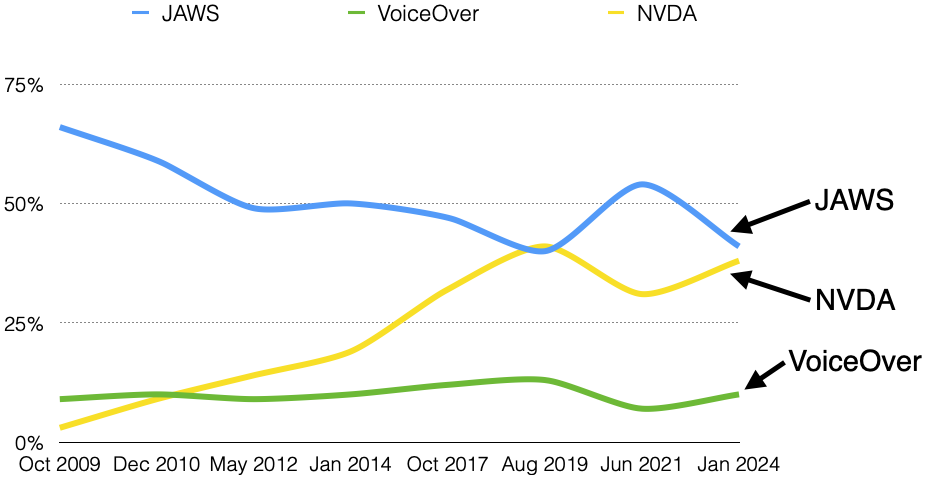
\includegraphics[max size={\linewidth}{\textheight}]{./assets/figures/screen-reader-trend.png}
  \captionsetup{justification=centering}
  \caption[Trend používání populárních odečítačů obrazovky]{Trend používání populárních odečítačů obrazovky~\cite{webaim-survey-2024}}
  \label{fig:}
\end{figure}

V rámci práce budu testovat komponenty s VoiceOver, protože s tímto odečítačem obrazovky mám nejvíce zkušeností a z rozsahu práce a časové dotace je testování všech populárních odečítačů nemožné.

Důležitá poznámka k testování komponent pomocí odečítačů obrazovky je, že tyto testy zatím nejdou plně automatizovat.
Je důležitá interpretace výstupu odečítače obrazovky člověkem, protože podobně jako ve vytváření uživatelských rozhraní je důležité jak uživatel chápe výstup aplikace.

\section{APG}

\gls{apg}\footnote{\url{https://www.w3.org/WAI/ARIA/apg}} je soubor nejčastějších návrhových vzorů a \textit{widgetů}\footnote{V kontextu této práce je widget to samé jako komponenta} vyskytujících se na webu.
Každý widget má svoji vlastní stránku s popisem, účelem, klávesovou navigací a používanými atributy, rolemi a stavy z \gls{waiaria}.
Kromě specifikace widgetů obsahuje i další praktická doporučení mezi která patří~\cite{apg}:

\begin{itemize}
  \item Používání orientačních bodů na stránce
  \item Používání přístupných názvu a popisků pro elementy
  \item Používání strukturovaných rolí
\end{itemize}

\gls{apg} je praktickým zdrojem pro tvorbu přístupných komponent, protože jsou zde popsány důležité informace jako použité role, vlastnosti, stavy z \gls{waiaria}.
Jsou zde i doporučení pro klávesovou navigaci a obecné informace o tom, jak by komponenta měla být použita.

\section{Závěr kapitoly}

Tato kapitola popsala principy přístupnosti na webu a její základní mechanismy.
Výčet důležitých poznatků pro další části práce je následující:

\begin{itemize}
  \item Vlastnosti, stavy a role z \gls{waiaria} jsou důležitou součástí přístupných rozhraní.
  \item Návrhové vzory z \gls{apg} jsou praktickým zdrojem pro tvorbu přístupných komponent.
  \item Je důležité neopomíjet alternativní způsoby ovládání.
  \item Testování čteček obrazovky bude provedeno pomocí VoiceOver na MacOS.
\end{itemize}
